\section{Results}

\begin{frame}
        \centering
        \huge Results
        \note{
	        \begin{itemize}
	        	\item Two data stream experiments
	        	\item One classic train/test on each training set and then the test set
		    \end{itemize}
		}
\end{frame}

\begin{frame}
	\begin{columns}
		\begin{column}{0.3\textwidth}
			\begin{itemize}
				\item Twitter.sentiment.appspot.com data stream
			\end{itemize}
		\end{column}
		\begin{column}{0.7\textwidth}  %%<--- here
			\begin{figure}
				\centering
				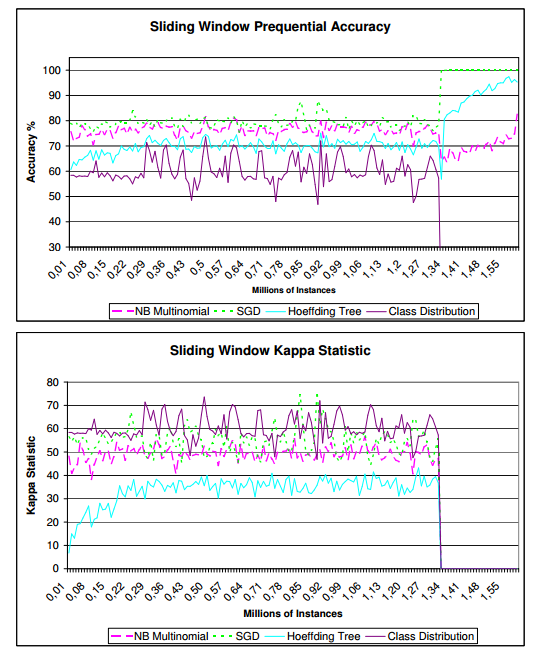
\includegraphics[scale=0.45]{sentimentdatastream.png}
			\end{figure}
		\end{column}
	\end{columns}
\end{frame}

\begin{frame}
	\begin{table}[htb]
		\centering
		\begin{tabular}{llll}
			\multicolumn{1}{c}{} 	& Accuracy 		& Kappa			& Time\\ \cmidrule{1-4}
			Multinomial Naïve Bayes	& \num{75.05}\%	& \num{50.10}\%	& \num{116.62} sec.\\
			SGD						& \num{82.80}\%	& \num{62.60}\%	& \num{219.54} sec.\\
			Hoeffding Tree			& \num{73.11}\%	& \num{46.23}\%	& \num{5525.51} sec.\\ \cmidrule{1-4}
		\end{tabular}
		\caption{Twittersentiment.appspot data stream}
	\end{table}
	\begin{table}[htb]
		\centering
		\begin{tabular}{lll}
			\multicolumn{1}{c}{} 	& Accuracy 		& Kappa\\ \cmidrule{1-3}
			Multinomial Naïve Bayes	& \num{82.45}\%	& \num{64.89}\%\\
			SGD						& \num{78.55}\%	& \num{57.23}\%\\
			Hoeffding Tree			& \num{69.36}\%	& \num{38.73}\%\\ \cmidrule{1-3}
		\end{tabular}
		\caption{Twittersentiment.appspot test dataset}
	\end{table}
\end{frame}


\begin{frame}
	\begin{columns}
		\begin{column}{0.3\textwidth}
			\begin{itemize}
				\item Edinburgh corpus data stream
			\end{itemize}
		\end{column}
		\begin{column}{0.7\textwidth}  %%<--- here
			\begin{figure}
				\centering
				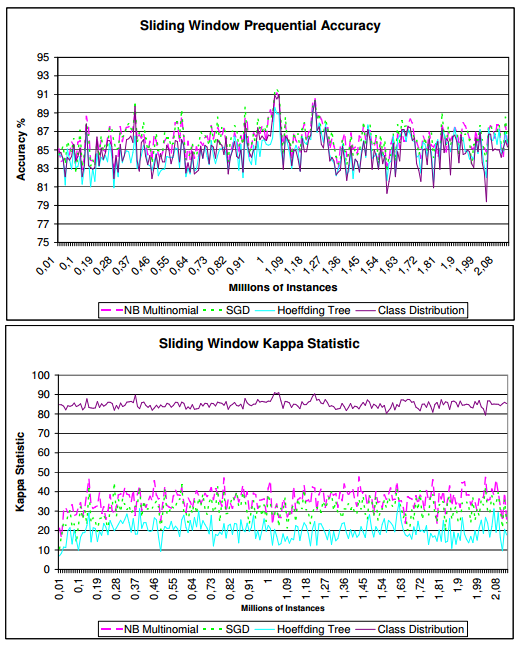
\includegraphics[scale=0.45]{edinburghdatastream.png}
			\end{figure}
		\end{column}
	\end{columns}
\end{frame}

\begin{frame}
	\begin{table}[htb]
		\centering
		\begin{tabular}{lll}
			\multicolumn{1}{c}{} 	& Accuracy 		& Kappa\\ \cmidrule{1-3}
			Multinomial Naïve Bayes	& \num{73.81}\%	& \num{47.28}\%\\
			SGD						& \num{67.41}\%	& \num{34.23}\%\\
			Hoeffding Tree			& \num{60.72}\%	& \num{20.59}\%\\ \cmidrule{1-3}
		\end{tabular}
		\caption{Accuracu and Kappa for twittersentiment.appspot.com using Edinburgh corpus as training data}
	\end{table}
\end{frame}

\begin{frame}
	\frametitle{Conclusion}
	\begin{itemize}
		\item SGD-based model is the recommended one for this data
	\end{itemize}
\end{frame}

\begin{frame}
	\frametitle{Future Work}
	\begin{itemize}
		\item Real time analysis
		\item Geographical place
		\item Followers
		\item Number of friends
	\end{itemize}
	\note{
		In future work, we would like to extend the results presented here by evaluating
		our methods in real time and using other features available in Twitter
		data streams, such as geographical place, the number of followers or the number
		of friends.
	}
\end{frame}